\documentclass[]{article}

\usepackage[italian]{babel}
\usepackage[margin=20mm, footskip = 20pt]{geometry}
\usepackage{array}
\usepackage{tabularx}
\usepackage{graphicx}
\usepackage{subfiles}
\usepackage{hyperref}
\usepackage{nameref}
\usepackage{titlesec}
\usepackage{longtable}
\usepackage[table]{xcolor}
\usepackage{titling}
\usepackage{lastpage}
\usepackage{ifthen}
\usepackage{calc}
\usepackage{soulutf8}
\usepackage{contour}
\usepackage{float}
\usepackage{fancyhdr}
\usepackage{multirow}
\usepackage{pgfgantt}
\usepackage{lscape}

\newcommand{\hr}{\par\vspace{-.1\ht\strutbox}\noindent\hrulefill\par}

\graphicspath{ {./}
	{./commons/res}
}

%--------------------------------------------------
% Comandi per inserire contenuto del documento
%--------------------------------------------------
\makeatletter

\newcommand\appendToGraphicsPath[1]{%
	\g@addto@macro\Ginput@path{{#1}}%
}

\newcommand{\setTitle}[1]{%
	\newcommand{\@phTitle}{#1}%
}
\newcommand{\phTitle}{\@phTitle}

\newcommand{\setDate}[1]{%
	\newcommand{\@phDate}{#1}%
}
\newcommand{\phDate}{\@phDate}

\newcommand{\setUso}[1]{%
	\newcommand{\@uso}{#1}%
}
\newcommand{\uso}{\@uso}

\newcommand{\setVersione}[1]{%
	\newcommand{\@versione}{#1}%
}
\newcommand{\versione}{\@versione}

\newcommand{\disabilitaVersione}{%
	\renewcommand{\setVersione}[1]{}%
	\renewcommand{\versione}{DISABILITATA}
}

\newcommand{\setResponsabile}[1]{%
	\newcommand{\@responsabile}{#1}%
}
\newcommand{\responsabile}{\@responsabile}

\newcommand{\setRedattori}[1]{%
	\newcommand{\@redattori}{#1}%
}
\newcommand{\redattori}{\@redattori}

\newcommand{\setVerificatori}[1]{%
	\newcommand{\@verificatori}{#1}%
}
\newcommand{\verificatori}{\@verificatori}

\newcommand{\setModifiche}[1]{%
	\newcommand{\@modifiche}{#1}%
}
\newcommand{\modifiche}{\@modifiche}

\makeatother 

%--------------------------------------------------
% Comandi per i documenti esterni e il glossario
%--------------------------------------------------

\newcommand{\dext}[1]{\textsc{#1\textsubscript{\textit{D}}}}

\newcommand{\glock}[1]{\textsc{#1\textsubscript{\textit{G}}}}

%--------------------------------------------------
% Comandi per impostare sottotitoli di quarto e quinto livello
%--------------------------------------------------

\setcounter{secnumdepth}{4}
\setcounter{tocdepth}{4}

\titleformat{\paragraph}
{\normalfont\normalsize\bfseries}{\theparagraph}{1em}{}
\titlespacing*{\paragraph}{0pt}{2.25ex plus 1ex minus .2ex}{1.5ex plus .2ex}

\titleformat{\subparagraph}
{\normalfont\normalsize\bfseries}{\thesubparagraph}{1em}{}
\titlespacing*{\subparagraph}{0pt}{1.75ex plus 1ex minus .2ex}{.75ex plus .1ex}

\appendToGraphicsPath{../../commons/res/}

%------------------------------
%
% COMANDI DI CONFIGURAZIONE
%
%------------------------------

\setTitle{Piano di Qualifica}

\setVersione{0.0.2}

\setDate{04-01-2021}

\setResponsabile{Valton Tahiraj}

\setRedattori{
    Alessandro Chimetto\\&
    Valton Tahiraj
}

\setVerificatori{ Giacomo Bulbarelli \\&
	Valton Tahiraj
}

\setUso{Esterno}

\setModifiche{
	0.0.2 & Valton Tahiraj & Verificatore & 03-01-2021 & Verifica modifica struttura documento \\
    0.0.2 & Alessandro Chimetto & Amministratore & 03-01-2021 & Modifica struttura documento\\
    0.0.1 & Giacomo Bulbarelli & Verificatore & 31-12-2020 & Verificata prima stesura \\
	0.0.1 & Valton Tahiraj & Amministratore & 31-12-2020 & Prima stesura
}

\begin{document}

	% Direttive per la creazione del titolo tramite comando maketitle
\title{\huge \textsc{\phTitle{}} \\
	\vspace{11pt} \large \textsc{\phDate{}}}

\author{} % Non toccare
\date{} % Non toccare

%--------------------
% Frontespizio
%--------------------

% Logo del gruppo
\begin{figure}[t!]
	\centering
	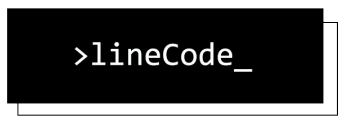
\includegraphics[width=20em]{lclong}
\end{figure}

% Titolo / Nome
\maketitle
\thispagestyle{empty}

% Dati specifici sul doc in forma tabulare
\begin{table}[ht]
	\begin{center}
		\label{tab:Dati sul documento}
		\begin{tabular}{r|l}
			\multicolumn{2}{c}{ \textsc{Dati sul documento} } \\
			\hline
			\textbf{Versione} & \versione{} \\
			\textbf{Uso} & \uso{}  \\
			\textbf{Redattori} & \redattori{} \\
			\textbf{Verificatori} & \verificatori{} \\
			\textbf{Responsabile} & \responsabile{} \\
			\textbf{Destinatari} & lineCode \\
								& prof.\ Vardanega Tullio \\		
								& prof.\ Cardin Riccardo \\
			\ifthenelse{\equal{\uso}{Esterno}}{
								& Sanmarco Informatica
			}{} \\
		\end{tabular}
	\end{center}
\end{table}

\newpage

\renewcommand{\arraystretch}{2} % allarga le righe con dello spazio sotto e sopra
\begin{longtable}[H]{>{\centering\bfseries}m{2cm} >{\centering}m{3.5cm} >{\centering}m{2.5cm} >{\centering}m{3cm} >{\centering\arraybackslash}m{5cm}}
	\rowcolor{lightgray}
	{\textbf{Versione}} & {\textbf{Nominativo}} & {\textbf{Ruolo}} & {\textbf{Data}} & {\textbf{Descrizione}}  \\
	\endfirsthead%
	\rowcolor{lightgray}
	{\textbf{Versione}} & {\textbf{Nominativo}}  & {\textbf{Ruolo}} & {\textbf{Data}} & {\textbf{Descrizione}}  \\
	\endhead%
	\modifiche{}%
\end{longtable}
	\newpage

	%--------------------------------
	%
	% IL CONTENUTO INIZIA DA QUI
	%
	%--------------------------------

	\section{Introduzione}
	\subsection{Scopo del documento}
Il documento ha lo scopo di definire le guidelines del way of working adottato dal team lineCode. Le attività presenti in questo documento sono redatte da processi contenuti nello standard ISO/IEC 12207:1995. Risulta quindi necessario che tutti i membri del gruppo prendano visione di questo documento ai fini di coesione e uniformità all'interno del progetto.

\subsection{Scopo del prodotto}
Il \glock{capitolato} C5 ha come obbiettivo la realizzazione di un applicativo \glock{Real-Time} in grado di guidare delle unità dotate di mobilità autonoma in ambienti specifici, partendo dal presupposto che queste si muovano in ambienti in cui sono presenti altre unità (autonome o meno).

\subsection{Glossario e documenti esterni}
In supporto alla documentazione viene fornito un glossario per chiarire, con una definizione, eventuali termini specifici contenuti in questo documento.
Saranno adottati quindi questi due simboli a pedice:
\begin{itemize}
	\item \textit{D} se indicano un documento specifico;
	\item \textit{G} se incluse nel \dext{glossario}.
\end{itemize}

\subsection{Riferimenti}
	\subsubsection{Riferimenti normativi}
	\begin{itemize}
		\item \textbf{{C5 - PORTACS}}: \url{https://www.math.unipd.it/~tullio/IS-1/2020/Progetto/C5.pdf};
        \item \textbf{Oracle Java Code Conventions}: \url{https://www.oracle.com/technetwork/java/codeconventions-150003.pdf};
        \item \textbf{Angular coding style guide}: \url{https://angular.io/guide/styleguide}.
	\end{itemize}
	\subsubsection{Riferimenti informativi}
	\begin{itemize}
		\item \textbf{ISO/IEC 12207:1995}: \url{https://www.math.unipd.it/~tullio/IS-1/2009/Approfondimenti/ISO_12207-1995.pdf};
		\item \textbf{Gitflow}: \url{http://nvie.com/posts/a-successful-git-branching-model/};
		\item \textbf{Documentazione Zapier}: \url{https://zapier.com/help};
		\item \textbf{Documentazione act}: \url{https://github.com/nektos/act/blob/master/README.md};
		\item \textbf{Studio di Fattibilità}: \dext{Studio di Fattibilità v1.0.0};
		\item \textbf{Piano di Qualifica}: \dext{Piano di Qualifica v2.0.0};
		\item \textbf{Piano di Progetto}: \dext{Piano di Progetto v2.0.0}.
	\end{itemize}
	\subsection{Scopo del documento}
	
	
	\subsection{Scopo del prodotto}
	
	\subsection{Glossario e Documenti esterni}
	
	\subsection{Riferimenti}
	
	\subsubsection{Normativi}
	
	\subsubsection{Informativi}
	
	
	\newpage

	\section{Qualità di processo}
	

\subsubsection{Introduzione}
Durante lo svolgimento del progetto sono stati identificati e perseguiti criteri di qualità al fine di realizzare un prodotto efficace. \\
Tali criteri permettono un miglioramento continuo tramite il monitoraggio e la stima degli stessi.\\
All'interno del documento \dext{Norme di Progetto v1.0.0}, sezione Processi Organizzativi, paragrafo 7.1.9; sono stati identificati i criteri necessari che verranno qui di seguito analizzati.
\subsubsection{Metriche}

\begin{table} [h!]
	\rowcolors{2}{gray!25}{gray!6}
	\begin{center}
		\begin{tabular} {m{2 cm} m{7 cm} c c }
			\rowcolor{lightgray}
			\textbf{ID} & \textbf{Nome}& \textbf{Valore Accettabile} & \textbf{Valore Ottimale}\\
			MP01 & Schedule Variance (SV)   & $\geq$ -5\%    & 0\% \\
			MP02 & Budgeted Cost of Work Performed (BCWP) & //           & // \\
			MP03 & Budgeted Cost of Work Scheduled (BCWS) & //           & // \\
			MP04 & Cost Variance (CV)   & $\geq$ -5\% & 0\% \\
			MP05 & Actual Cost of Work Performed (ACWP) & //           & // \\
			MP06 & Unbudgeted Risks (UR)   & $\leq$ 5 rischi & 0 rischi\\
			MP07 & Defects Removal Efficiency (DRE)  & $\geq$  80\% & 100\%\\

		\end{tabular}
	\caption{Metriche qualità di processo}
	\end{center}
\end{table}






	\newpage

	\section{Qualità di prodotto}
	Per garantire e valutare la qualità del prodotto, il gruppo ha deciso di fare riferimento allo standard ISO/IEC 9126, il quale definisce i parametri per produrre un prodotto di buona qualità ed il raggiungimento di tale caratteristica. \\
Oltre alle qualità presenti nello standard sopra citato, il gruppo ha deciso di utilizzare altri parametri per quantificare la qualità della documentazione fornita con il prodotto software; le quali, riportate di seguito.

\subsection{Qualità dei documenti}

\subsubsection{Comprensione}
Tutti i documenti devono essere leggibili e comprensibili.\\
Queste qualitá derivano dalla correttezza lessicografica, grammaticale e semantica.

\subsubsection{Obiettivi}
\begin{itemize}
    \item \textbf{leggibilità:}per garantire la leggibilità dei documenti si è deciso di utilizzare \glock{l'indice di gulpease} come indicatore per questa caratteristica;
    \item \textbf{correttezza:} i documenti presentati non devono contenere errori ortografici di alcun genere.
\end{itemize}

\subsubsection{Metriche}

\begin{table} [h!]
	\rowcolors{2}{gray!25}{gray!6}
	\begin{center}
		\begin{tabular} {m{2 cm} m{7 cm} c c }
			\rowcolor{lightgray}
			\textbf{ID} & \textbf{Nome}& \textbf{Valore Accettabile} & \textbf{Valore Ottimale}\\
			MD01 & Indice di Gulpease  		 & $\geq$ 40\%    			& $\geq$ 60\% \\
			MD02 & Correttezza ortografica 				&0						&0
		\end{tabular}
	\caption{Metriche qualità di prodotto}
	\end{center}
\end{table}
	\newpage

	\section{Test}
	
La classificazione dei test è riportata alla sezione Verifica delle \dext{Norme di progetto v2.0.0}. \\

\subsection{Tipologie di test}
I test saranno di quattro tipologie:
\begin{itemize}
	\item \textbf{Test di Sistema [TS] };
	\item \textbf{Test di Accettazione [TA]};
	\item \textbf{Test di Integrazione [TI]};
	\item \textbf{Test di Unità [TU]}.\\
\end{itemize}

\subsubsection{Test di sistema}

	\newcommand*{\thead}[1]{\multicolumn{1}{c}{\bfseries #1}}	
	\rowcolors{2}{gray!6}{gray!25}
	\setlength{\tabcolsep}{10pt}
	\begin{longtable}[h!] { c  m{12cm} c}
		\caption{Test di Sistema} \\
		\rowcolor{lightgray}
		\thead{Test}  & \thead{Descrizione} & \thead{Esito} \\ \endhead%
	
		TSMF1   & La mappa deve essere disponibile per l'utente generico in sola lettura	& NI \\
		
		TSMF1.1 & L'utente generico deve poter visualizzare la legenda dei simboli utilizzati all'interno della mappa & NI \\
		
		TSFM1.2 & La mappa deve aggiornarsi periodicamente, mostrando le informazioni sul movimento delle unità che fanno parte del sistema & NI\\
		
		TSDM1.3 & La mappa deve mostrare le informazioni sui pedoni che comunicano con il sistema & NI \\
		
		TSFM1.4 & La mappa deve essere visualizzabile per ogni tipo di utente & NI\\
		
		
		TSFM2   & L'utente registrato deve poter effettuare il login. All'utente viene chiesto di:
				\begin{itemize}
					\item accedere all'area login;
					\item inserire il nome utente;
					\item inserire la password.
				\end{itemize}
								& NI \\
								
		TSFM2.1 & L'utente deve visualizzare un messaggio di errore nel caso in cui:
					\begin{itemize}
						\item viene fornito un nome utente non esistente;
						\item viene fornita una password errata.
					\end{itemize}
									& NI \\		
		TSFM3   & L'utente autenticato deve poter effettuare il logout dal sistema. L'utente può verificare che la disconnessione sia avvenuta con successo & NI \\
		
		TSFM4   & La guida utente deve essere visualizzabile dai soli utenti registrati & NI \\
									
		TSFM4.1 & La guida utente deve contenere tutte le istruzioni che un utente può svolgere all'interno del sistema & NI \\
		
		TSFM5   & L'utente autenticato deve poter visualizzare la lista delle unità attive con il proprio ID & NI \\
		
		TSFM5.1 & Ogni elemento della lista di unità fornisce un ambiente grafico per la gestione delle proprietà dell'unità selezionata & NI \\
		
		TSFO5.2 & L'utente autenticato, dentro l'ambiente grafico, deve visualizzare l'ID dell'unità selezionata & NI \\
		
		TSFM5.3 & L'utente autenticato deve poter visualizzare le seguenti informazioni dell'unità:
					\begin{itemize}
						\item le coordinate della posizione attuale all'interno della mappa;
						\item lo stato in cui si trova;
						\item la velocità attuale;
						\item la direzione del prossimo passo suggerita dal sistema;
						\item la coda degli ordini assegnati.
					\end{itemize}	
									&NI\\
				
		TSFM5.4  & L'utente autenticato deve poter impartire i seguenti comandi all'unità:
					\begin{itemize}
						\item \underline{Start};
						\item \underline{Stop};
						\item \underline{Go Back};
						\item \underline{Shutdown}.
					\end{itemize}
									& NI \\
									
		TSFM5.5  & L'utente autenticato deve poter aggiungere un nuovo ordine alla coda degli ordini assegnati all'unità & NI\\
		
		TSFM5.6  & L'utente autenticato deve poter eliminare un ordine alla coda degli ordini assegnati all'unità & NI\\
		
		TSFM6 & L'amministratore deve poter visualizzare la lista degli utenti registrati, con le seguenti informazioni:
					\begin{itemize}
						\item nome utente;
						\item password.	
					\end{itemize}
									& NI \\
		TSFM6.1 & L'amministratore deve poter creare un nuovo utente. Il sistema richiede in input le seguenti credenziali:
					\begin{itemize}
						\item nome utente;
						\item password;
						\item status.
					\end{itemize}
										& NI \\
										
		TSFM6.2  & L'amministratore deve poter modificare un utente registrati. Il sistema richiede in input le seguenti credenziali:
					\begin{itemize}
						\item nome utente;
						\item password.
					\end{itemize}
											& NI \\
		TSFM6.3 & L'amministratore deve poter eliminare un utenti registrato & NI \\
		
		TSFM6.4 & L'amministratore deve visualizzare un messaggio di errore nel caso in cui:
						\begin{itemize}
						\item il nome utente inserito sia già esistente; 
						\item la password non è formattata correttamente.
					\end{itemize}
										& NI \\
		TSFM7   & L'amministratore per poter modificare la mappa, deve poter inserire un file da validare & NI\\
		
		TSFM7.1 & L'amministratore deve visualizzare un messaggio di errore nel caso in cui il file non sia formattato correttamente & NI \\
		
		TSFM8   & L'amministratore deve poter visualizzare la lista delle unità registrate, con il proprio ID & NI\\
		
		TSFM8.1 & L'amministratore deve poter aggiungere una nuova unità alla liste delle unità registrate. Il sistema richiede in input l'ID & NI\\	
		
		TSFM8.2 & 	L'amministratore deve poter modificare la lista delle unità registrate. Il sistema richiede in input il rispettivo ID & NI\\
		
		TSFM8.3 & L'amministratore deve poter eliminare una unità dalla lista & NI\\
		
		TSFM8.4  & L'amministratore deve visualizzare un messaggio d'errore nel caso venga fornito un ID già esistente & NI \\
		
		TSFM9   & L'unità, dotata di sensoristica, deve comunicare al sistema la posizione relativa degli ostacoli che riescono a rilevare & NI \\
		
		TSFM10 & Il sistema deve ricevere le coordinate dall'unità sulla sua posizione attuale & NI \\
		
		TSFM11 & L'unità deve avere un percorso fornito dal sistema per raggiungere il prossimo \glock{POI} & NI \\
		
		TSFM12 & L'unità deve avere una lista di \glock{POI} da raggiungere & NI \\
		
		TSFM13  & L'utente autenticato può modificare la lista deglli ordini solo quando l'unità si trova in una base di ricarica & NI \\
		
		TSFM14  & L'unità, con coda degli ordini vuota, deve ritornare nella base di ricarica & NI \\
		
		TSFM15  & L'unità non può superare un certo limite di velocità & NI \\
		
		TSFM16 & L'unità può assumere uno dei seguenti stati:
				\begin{itemize}
					\item \underline{Going to X};
					\item \underline{Stop};
					\item \underline{Base};
					\item \underline{Error Y}.
				\end{itemize}		
										& NI \\
										
		TSFM17  & Il sistema dispone di un algoritmo che deve:
				\begin{itemize}
					\item calcolare il percorso che l'unità deve percorrere per raggiungere il \glock{POI};
					\item evitare la collisione con altre unità;
					\item evitare la collisione con gli ostacoli.
				\end{itemize}		
										& NI \\
		
		TSFO18  & Il percorso restituito dall'algoritmo, è un percorso ottimo & NI\\
		
		TSFD19 & Il sistema riceve dal pedone le informazioni sulla sua posizione & NI\\

		TSFD20  & Il sistema riconosce il pedone come un ostacolo & NI \\
		\hline
		
		TSMC1   & Deve essere fornito un documento con i casi d'uso in formato UML & NI \\
		
		TSMC2   & Deve essere consegnato uno schema relativo al design della base di dati & NI \\
		
		TSMC3  &Deve essere consegnata la documentazione delle \glock{API} realizzate & NI\\
		
		TSMC4   & Deve essere consegnata una lista di bug risolti durante lo sviluppo & NI\\
		
		TSMC5   & Il codice sorgente del prodotto dovrà essere versionato con \glock{GitHub} & NI\\
		
		TSMC6   & Ogni entità sviluppata facente parte del sistema dovrà essere contenuta in un container \glock{Docker} & NI \\
		
		TSMC7   & Deve essere fornito un \glock{Dockerfile} contenente:
						\begin{itemize}
							\item il motore di calcolo;
							\item il visualizzatore \glock{Real-Time}.
						\end{itemize} 
											& NI \\
											
		TSMC7.1 & Deve essere fornito un \glock{Dockerfile} per la singola unità & NI \\
		
		TSD7.2 &  Deve essere fornito un \glock{Dockerfile} per il singolo pedone & NI \\
		
		TSMC8  & L'astrazione della mappatura dell'ambiente dovrà rispettare una struttura a griglia con divisione in celle & NI \\
		
		\hline
		
		TSMQ1 & Il prodotto va rilasciato con la licenza \glock{open-source} più aperta possibile in base alle librerie utilizzate & NI \\
		
		TSMQ2 & Il prodotto deve essere conforme con quanto dichiarato nel documento \dext{ Piano di Qualifica v2.0.0} & NI \\
		
		TSMQ3  & Devono essere realizzati test di unità e di integrazione per vericare le singole componenti del prodotto & NI \\
		
		\hline
		
		TSMP1  &  Il tempo di aggiornamento della mappatura rispetto alla posizione delle unità nell'ambiente deve essere $\geq$ 5 secondi & NI \\
	
		TSDP1.1  & Il tempo di aggiornamento della mappatura rispetto alla posizione delle unità nell'ambiente deve essere $\geq$ 2.5 secondi & NI \\
		
		TSOP1.2  &  Il tempo di aggiornamento della mappatura rispetto alla posizione delle unità nell'ambiente deve essere $\geq$ 1 secondi & NI \\
										
		TSMP2	& Il servizio non deve mai essere interrotto secondo una logica di \glock{zero downtime}	& NI \\\\									
\end{longtable}

\subsubsection{Test di accettazione}
I test di Accettazione hanno lo scopo di dimostrare che il prodotto sviluppato soddisfi i requisiti presenti nel capitolato e concordati con il proponente e, con quest'ultimo, eseguito durante il collaudo finale del prodotto. 

\subsubsection{Test di integrazione}
Le specifiche di questi test verranno scritte successivamente rispettando il \glock{Modello a V}.
\subsubsection{Test di Unità}
Le specifiche di questi test verranno scritte successivamente rispettando il \glock{Modello a V}.





	\newpage
	
	\section{Resoconto di verifica}
	\subsection{Verifica della documentazione}
	Per la verifica della documentazione si utilizza la tecnica del \glock{walkthrough} revisionando i documenti per intero e la tecnica di \glock{inspection}. 

\subsubsection{Calcolo leggibilità e controllo ortografia dei documenti}
	Per verificare quanto sono leggibili i documenti redatti si utilizza l'\glock{indice di gulpease} ed è stato effettuato un controllo di ortografia. La seguente tabella contiene i risultati ottenuti durante il periodo trascorso dall'ultima revisione:

\begin{table} [h!]
	\rowcolors{2}{gray!25}{gray!6}
	\begin{center}
		\begin{tabular} { c c c c}
			\rowcolor{lightgray}
			\textbf{Documento}&\textbf{Errori ortografici}&\textbf{Indice di gulpease}&\textbf{Esito}\\
			\dext{Piano di progetto v1.0.0}		& 0 & 0  &Superato\\
			\dext{Norme di progetto v1.0.0} 	& 0	& 0  &Superato\\
			\dext{Studio di fattibilità v1.0.0}	& 0	& 0  &Superato\\
			\dext{Glossario v1.0.0}				& 0	& 0  &Superato\\
			\dext{Piano di qualifica v1.0.0}	& 0	& 0  &Superato\\
			\dext{Media verbali v1.0.0}			& 0	& 0  &Superato\\
			\dext{Analisi dei requisiti v1.0.0}	& 0	& 0  &Superato\\
		\end{tabular}
	\end{center}
	\caption{Esiti verifiche automatizzate - Revisione di Progettazione}
\end{table}

\noindent Con i seguenti grafici, illustriamo l'andamento dell'indice di gulpease e degli errori ortografici riscontrati per ogni documento, nelle revisioni effettuate:
\begin{figure}[H]
	\centering
	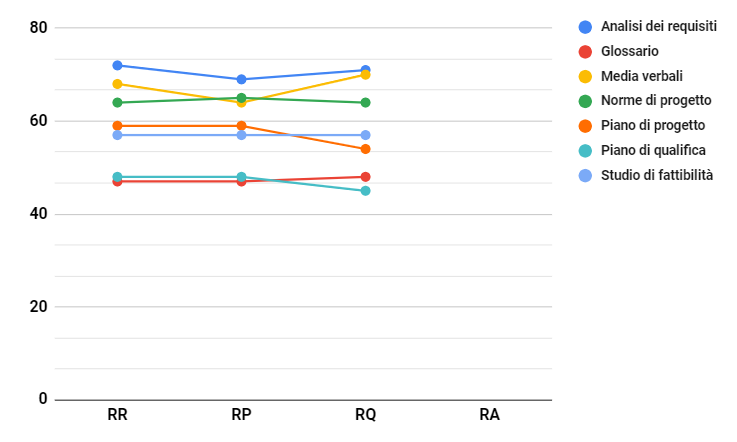
\includegraphics[width=12cm]{images/gulpease.png}
	\caption{Indice di gulpease per revisione}
\end{figure}
\begin{figure}[H]
	\centering
	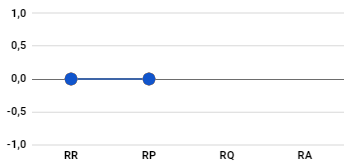
\includegraphics[width=8cm]{images/err_ortografici.png}
	\caption{Errori ortografici per revisione}
\end{figure}

\subsection{MP01 - Schedule Variance}
Con la seguente metrica si tiene traccia di eventuali anticipi (\textit{numero positivo}) o ritardi (\textit{numero negativo}) rispetto alla schedulazione delle attività di progetto pianificate.
%\begin{figure}[H]
%	\centering
%	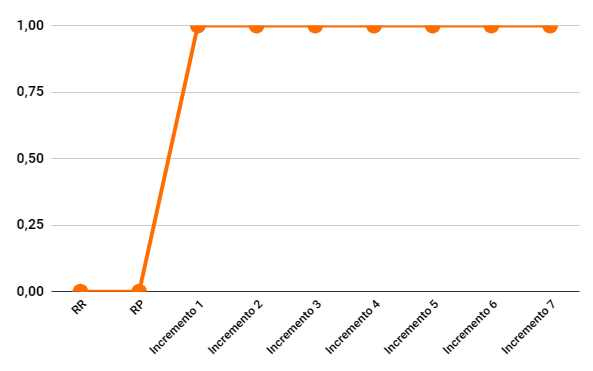
\includegraphics[width=8cm]{images/unbudgeted_risks.png}
%	\caption{Unbudgeted risks per revisione}
%\end{figure}

\subsection{MP04 - Cost Variance - CV}
Con la seguente metrica verifica se il valore del costo realmente maturato è maggiore, uguale o minore rispetto al costo effettivo.
%\begin{figure}[H]
%	\centering
%	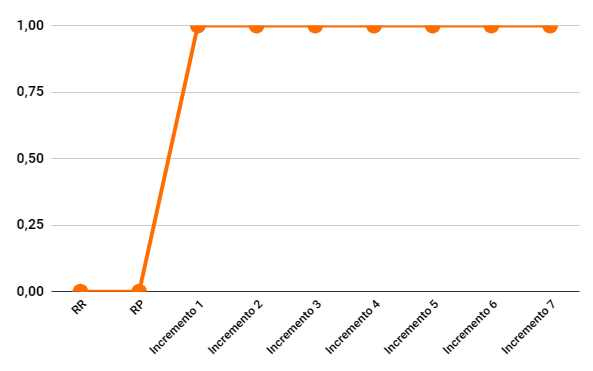
\includegraphics[width=8cm]{images/unbudgeted_risks.png}
%	\caption{Unbudgeted risks per revisione}
%\end{figure}

\subsection{MP06 - Unbudgeted risks}
Data la possibilità di incontrare rischi, non preventivati in fase di analisi, di seguito verranno illustrate tali evenienze per ogni revisione del progetto:
%\begin{figure}[H]
%	\centering
%	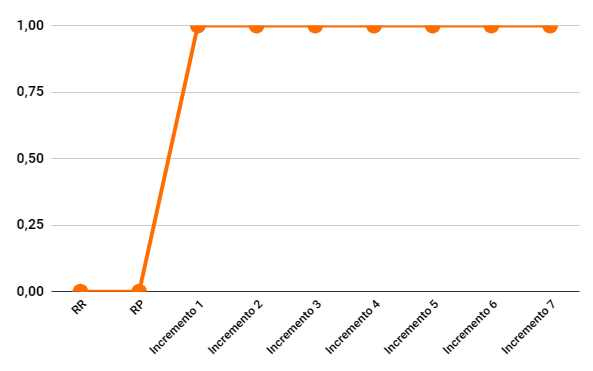
\includegraphics[width=8cm]{images/unbudgeted_risks.png}
%	\caption{Unbudgeted risks per revisione}
%\end{figure}

	\newpage
	
	\section{Valutazioni di miglioramento}
	Questa sezione si focalizza sul miglioramento della produttività dei \glock{processi} coinvolti nella
realizzazione del prodotto descritto nel \glock{capitolato} scelto. Essendo il primo progetto realistico affrontato dai membri del gruppo, problemi di natura organizzativa interna, di adempimento efficace
dei ruoli assegnati e di giusto utilizzo degli strumenti scelti sono dietro l’angolo. Per far fronte a queste
possibili problematiche e cercare di migliorare in maniera costante la produttività del gruppo, verranno elencati i problemi più grandi rilevati e le relative contromisure, man mano che saranno identificati
nel corso della realizzazione del prodotto.

\subsection{Valutazioni sull'organizzazione}
\begin{table} [h!]
	\rowcolors{2}{gray!25}{gray!6}
	\begin{center}
		\begin{tabular} { m{8cm} m{8cm}  }
			\rowcolor{lightgray}
			\textbf{Problema rilevato} & \textbf{Contromisura}\\
			Nei primi mesi di lavoro è stato difficile trovarsi data la attuale situazione di emergenza globale. & E' stato creato un canale \glock{discord} per garantire una comunicazione testuale e vocale costante tra alcuni o tutti i membri del gruppo.
			
		\end{tabular}
	\end{center}
	\caption{Tabella contenente le valutazioni sull’organizzazione}
\end{table}

\newpage
\subsection{Valutazioni sui ruoli}
\begin{table} [h!]
	\rowcolors{2}{gray!25}{gray!6}
	\begin{center}
		\begin{tabular} { m{3cm} m{7cm} m{6cm} }
			\rowcolor{lightgray}
			\textbf{Ruolo} & \textbf{Problema rilevato} & \textbf{Contromisura}\\
			Responsabile & Durante la fase relativa alla stesura dei documenti per proporsi ufficialmente come fornitori per il capitolato, i compiti sono stati assegnati dal responsabile su base volontaria, portando così a situazioni in cui alcuni membri si sono ritrovati sovraccarichi di lavoro
			mentre altri erano tenuti a svolgere attività più sbrigative. Questo fatto ha portato alcuni colleghi a chiedere una ridistribuzione dei compiti.& Dopo ogni assegnazione di compiti da svolgere, il responsabile di turno si deve impegnare a ricontrollare se sono stati spartiti equamente tra i membri, cosicchè non si subiscano rallentamenti per via di ridistribuzioni degli oneri di progetto. \\			
			Analista & 	Essendo il compito dell'analista quello di guidare il gruppo nel migliorare processi, prodotti, servizi e software attraverso l'analisi dei dati è stato difficile inizialmente coordinarsi efficientemente con gli altri membri del gruppo. & Gli analisti hanno deciso di svolgere quest’attività scambiandosi continuamente i propri risultati e chiedendo chiarimenti agli altri quando necessario.\\
			Verificatori &	Data l’inesperienza dei membri nell’attività di stesura dei documenti, è indispensabile che i verificatori controllino ogni sezione scrupolosamente.	Per fare ciò però,  devono avere una buona conoscenza di tutte le tematiche trattate nella documentazione. & Per risolvere questi problemi, ai verificatori
			si è deciso di non assegnare altri compiti durante lo svolgimento del processo di verifica, in
			modo che avessero il tempo materiale per attuarlo nel modo più efficace possibile.\\
			Amministratore & Per redarre alcune sezioni di certi documenti, i membri che hanno ricoperto questo ruolo hanno trovato delle difficoltà relative alla mancata presenza di materiale autorevole e chiaro che le descrivesse. & Si è deciso di prendere spunto dalla documentazione prodotta dai colleghi degli anni passati, confrontarla con quanto appreso durante il corso di ingegneria del software e procedere alla loro stesura cercando di trattare ogni sezione in modo approfondito e chiaro.
		\end{tabular}
\end{center}
\caption{Tabella contenente le valutazioni sui ruoli}
\end{table}

\newpage
\subsection{Valutazioni sgli strumenti}
\begin{table} [h!]
	\rowcolors{2}{gray!25}{gray!6}
	\begin{center}
		\begin{tabular} { m{2cm} m{7cm} m{7cm} }
			\rowcolor{lightgray}
			\textbf{Strumento} & \textbf{Problema rilevato} & \textbf{Contromisura}\\
			\glock{Version Control System} & Nel \glock{way of working} del particolare \glock{VCS} utilizzato, si sono fissate diverse regole su come condividere il materiale prodotto nel server. Queste regole non sono state attuate da alcuni membri, vista l’inesperienza, e ciò ha portato a rallentamenti nella fase di condivisione del materiale scelto per poter chiudere le \glock{milestone} relative e procedere ad aprire quelle successive. & E’ stato condiviso un documento testuale che spiega nel dettaglio come ottemperare alle regole scelte per l’utilizzo dello strumento, in modo da facilitare i membri più in difficoltà e non rendere il \glock{VCS} un ostacolo all’avanzamento del gruppo verso la realizzazione della documentazione necessaria. \\
			\LaTeX\ &	Questo strumento di scrittura è stato una novità per quasi tutti i membri del gruppo. All’inizio, in molti avevano errori di compilazione nei propri file, per cui non riuscivano a produrre opportuni file pdf. & Dopo il primo mese e mezzo dalla formazione del gruppo, i membri più esperti di \LaTeX\ hanno creato un template da utilizzare per la produzione della documentazione, riducendo ai minimi termini il numero di comandi da imparare per utilizzare questo software efficacemente.
		\end{tabular}
	\end{center}
\caption{Tabella contenente le valutazioni sugli strumenti}
\end{table}

	\newpage

\end{document}